%%%%%%%%%%%%%%%%%%%%%%%%%%%%%%%%%%%%%%%%%%%%%%%%%%%%%%%%%%%%%%%%%%%%
% Diskussion und Ausblick
%%%%%%%%%%%%%%%%%%%%%%%%%%%%%%%%%%%%%%%%%%%%%%%%%%%%%%%%%%%%%%%%%%%%

\chapter{React in der Praxis}
  \label{React in der Praxis}
\section{Entwicklungsumgebung}
\subsection{Nodejs}
Nodejs ist ein JavaScript Runtime Environment für die serverseitige Entwicklung mit JavaScript. Für Projekte mit React ist es vor allem wegen dem enthaltenen Paketmanager NPM wichtig. Dieser ist aktuell de-facto Standard zur Verteilung von Paketen in JavaScript und bietet die Möglichkeit die React-Applikation während der Entwicklung direkt über einen integrierten Webserver anzuzeigen. Ein weiterer wichtiger Vorteil von NPM ist die einfache Installation vieler Erweiterungsmodule, die spezielle Funktionen bieten und häufige Problemstellungen lösen können. \\
Der oben erwähnte Webserver ist die einfachste Möglichkeit eine React-Applikation außerhalb einer Produktionsumgebung anzuzeigen. Anders als bei statischen Webseiten ohne Skriptanteil, können dynamische Webseiten nicht ohne eine Server-Client-Umgebung aufgerufen werden. Grund dafür ist, dass der dynamische Inhalt erst beim Aufruf vom Server generiert wird. Soll die React-Applikation so angezeigt werden reicht dank NPM der kurze Befehl 'npm run start' um den Webserver zu starten und die Applikation anzuzeigen. Veränderungen im Code der Applikation werden dabei live compiliert, was die Fehlersuche und das Testen neuer Komponenten stark erleichtert. Wie in Abbildung 4.1 zu sehen ist, steht die Applikation unter einen lokalen URL zur Verfügung und könnte durch einen weiteren kurzen befehl 'npm run build' für die Produktion optimiert werden.
\begin{figure}[H]
     \centerline{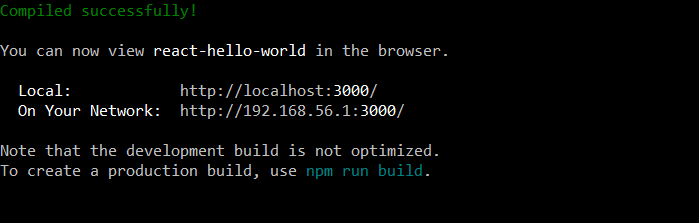
\includegraphics[width=14cm]{../Abbildungen/npmRunStart.png}}
  \caption{Laden von React (2 Zeilen) \& Button.js (1 Zeile)}
  \label{NPM Dialog}
\end{figure}
\subsection{Toolchains für React}
Für React ist eine Vielzahl von Toolchains zur Vereinfachung der Entwicklung verfügbar. Während es problemlos möglich ist ohne diese Werkzeug-Programme eine React Applikation zu entwickeln, sind sie in bestimmten Fällen sehr empfehlenswert. Besonders bei sehr große Projekte mit vielen Komponenten und/oder Drittpartei-Modulen sind entsprechende Toolchains wertvoll. Andere Vorteile sind die Vermeidung typischer Fehler im Projektaufbau und eine einfache Optimierung des Projekts für die Produktion.\\
Bekannte Toolchains sind unter anderem Create React App, Next.js und Gatsby. Create React App ist für die Entwicklung von single-page Applikationen wie dem LogikLehrtool-Projekt sehr gut geeignet. Next.js dagegen wird eher für die Entwicklung von serverseitig gerenderten Webseiten und Gatsby für statische Seiten verwendet. Darüber hinaus gibt es eine Vielzahl an weiteren Toolchains die sehr viele Anwendungsgebiete abdecken und auch für ungewöhnlichere Projekte eine passende Konfiguration erzeugen können.
\pagebreak
\section{React in HTML-Seiten einfügen}
Es ist sehr einfach React einer bestehenden HTML-Seite hinzuzufügen. Im folgenden Beispiel wird einer HTML-Seite ein Like-Button hinzugefügt.\\
\begin{figure}[thb]
     \centerline{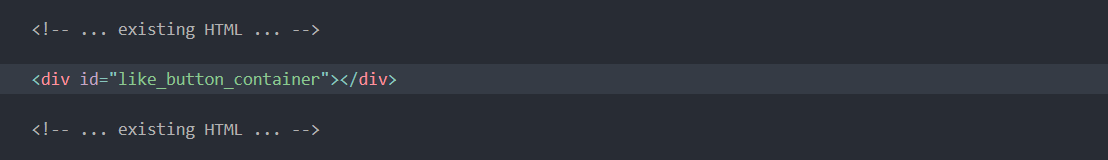
\includegraphics[width=14cm]{../Abbildungen/domContainer.png}}
  \caption{Erstellen eines Dom-Containers}
  \label{fig1_1}
  \vspace{1cm}
     \centerline{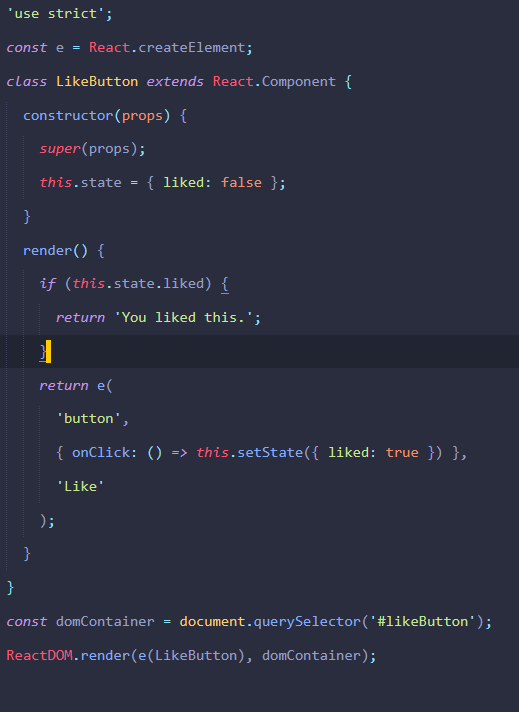
\includegraphics[width=8cm]{../Abbildungen/buttonScript.png}}
  \caption{Button.js: React-Script zur Verwendung des Dom-Containers}
  \label{fig1_1}
\end{figure}\\
Wie in Abbildung 4.1 zu sehen ist, wird als Erstes ein Dom-Container in der HTML-Datei eingefügt. Dieser Container wird anschließend bei der Erstellung eines React-Scripts mittels seiner ID verwendet. Abbildung 4.2 zeigt dieses Script, welches einen Button mit einer Klick-Reaktion erzeugt. Wird der Button geklickt, so ändert sich sein Status und es wird stattdessen der Satz 'You liked this' angezeigt. \\
Abschließend müssen in der HTML-Datei, wie in Abbildung 4.3,  nur noch die entsprechenden Skripte geladen werden. Dies beinhaltet zwei Skripte welche die React-Bibliothek laden und das eben erstellte Button-Skript welches unsere React-Komponente beinhaltet.
\begin{figure}[thb]
     \centerline{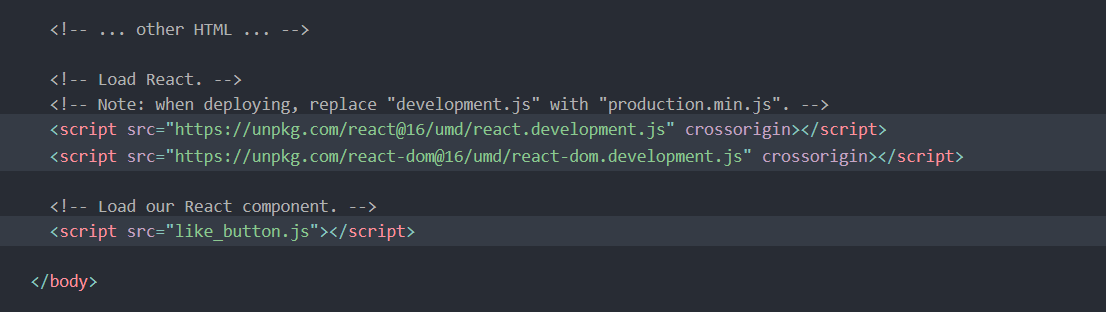
\includegraphics[width=14cm]{../Abbildungen/scriptLines.png}}
  \caption{Laden von React (2 Zeilen) \& Button.js (1 Zeile)}
  \label{fig1_1}
\end{figure}\\

